%%%%%%%%%%%%%%%%%%%%%%%%%%%%%%%%%%%%%%%%%%%%%%%%%%%%%%%%%%%%%%%%%%%%%%%%%%%%
% AGUJournalTemplate.tex: this template file is for articles formatted with LaTeX
%
% This file includes commands and instructions
% given in the order necessary to produce a final output that will
% satisfy AGU requirements, including customized APA reference formatting.
%
% You may copy this file and give it your
% article name, and enter your text.
%
%
% Step 1: Set the \documentclass
%
%

%% To submit your paper:
\documentclass[draft]{agujournal2019}
\usepackage{url} %this package should fix any errors with URLs in refs.
\usepackage{lineno}
\usepackage[inline]{trackchanges} %for better track changes. finalnew option will compile document with changes incorporated.
\usepackage{soul}
\usepackage[version=4]{mhchem}
\usepackage{natbib}

\linenumbers
%%%%%%%
% As of 2018 we recommend use of the TrackChanges package to mark revisions.
% The trackchanges package adds five new LaTeX commands:
%
%  \note[editor]{The note}
%  \annote[editor]{Text to annotate}{The note}
%  \add[editor]{Text to add}
%  \remove[editor]{Text to remove}
%  \change[editor]{Text to remove}{Text to add}
%
% complete documentation is here: http://trackchanges.sourceforge.net/
%%%%%%%

\draftfalse

%% Enter journal name below.
%% Choose from this list of Journals:
%
% JGR: Atmospheres
% JGR: Biogeosciences
% JGR: Earth Surface
% JGR: Oceans
% JGR: Planets
% JGR: Solid Earth
% JGR: Space Physics
% Global Biogeochemical Cycles
% Geophysical Research Letters
% Paleoceanography and Paleoclimatology
% Radio Science
% Reviews of Geophysics
% Tectonics
% Space Weather
% Water Resources Research
% Geochemistry, Geophysics, Geosystems
% Journal of Advances in Modeling Earth Systems (JAMES)
% Earth's Future
% Earth and Space Science
% Geohealth
%
% ie, \journalname{Water Resources Research}

\journalname{Geophysical Research Letters}


\begin{document}

%% ------------------------------------------------------------------------ %%
%  Title
%
% (A title should be specific, informative, and brief. Use
% abbreviations only if they are defined in the abstract. Titles that
% start with general keywords then specific terms are optimized in
% searches)
%
%% ------------------------------------------------------------------------ %%



\title{Antarctic Radiative and Temperature responses to a doubling of $\text{CO}_2$}

%% ------------------------------------------------------------------------ %%
%
%  AUTHORS AND AFFILIATIONS
%
%% ------------------------------------------------------------------------ %%

% Authors are individuals who have significantly contributed to the
% research and preparation of the article. Group authors are allowed, if
% each author in the group is separately identified in an appendix.)

% List authors by first name or initial followed by last name and
% separated by commas. Use \affil{} to number affiliations, and
% \thanks{} for author notes.
% Additional author notes should be indicated with \thanks{} (for
% example, for current addresses).

% Example: \authors{A. B. Author\affil{1}\thanks{Current address, Antartica}, B. C. Author\affil{2,3}, and D. E.
% Author\affil{3,4}\thanks{Also funded by Monsanto.}}

\authors{L. M. Freese\affil{1} and T. W. Cronin\affil{1}}

 \affiliation{1}{Department of Earth, Atmosphere and Planetary Sciences, Massachusetts Institute of Technology, Cambridge, Massachusetts, USA}
% \affiliation{2}{Second Affiliation}
% \affiliation{3}{Third Affiliation}
% \affiliation{4}{Fourth Affiliation}

\affiliation{=number=}{=Affiliation Address=}
%(repeat as many times as is necessary)

%% Corresponding Author:
% Corresponding author mailing address and e-mail address:

% (include name and email addresses of the corresponding author.  More
% than one corresponding author is allowed in this LaTeX file and for
% publication; but only one corresponding author is allowed in our
% editorial system.)

% Example: \correspondingauthor{First and Last Name}{email@address.edu}

\correspondingauthor{=name=}{=email address=}

%% Keypoints, final entry on title page.

%  List up to three key points (at least one is required)
%  Key Points summarize the main points and conclusions of the article
%  Each must be 100 characters or less with no special characters or punctuation and must be complete sentences

% Example:
% \begin{keypoints}
% \item	List up to three key points (at least one is required)
% \item	Key Points summarize the main points and conclusions of the article
% \item	Each must be 100 characters or less with no special characters or punctuation and must be complete sentences
% \end{keypoints}

\begin{keypoints}
\item enter point 1 here
\item enter point 2 here
\item enter point 3 here
\end{keypoints}

%% ------------------------------------------------------------------------ %%
%
%  ABSTRACT and PLAIN LANGUAGE SUMMARY
%
% A good Abstract will begin with a short description of the problem
% being addressed, briefly describe the new data or analyses, then
% briefly states the main conclusion(s) and how they are supported and
% uncertainties.

% The Plain Language Summary should be written for a broad audience,
% including journalists and the science-interested public, that will not have 
% a background in your field.
%
% A Plain Language Summary is required in GRL, JGR: Planets, JGR: Biogeosciences,
% JGR: Oceans, G-Cubed, Reviews of Geophysics, and JAMES.
% see http://sharingscience.agu.org/creating-plain-language-summary/)
%
%% ------------------------------------------------------------------------ %%

%% \begin{abstract} starts the second page

\begin{abstract}
[ Greenhouse gases (GHGs), such as $\ce{CO_2}$, impact global and local outgoing longwave radiation (OLR). The Antarctic is known for its a strong near-surface temperature inversion, where the addition of GHGs can lead to increased OLR during all but the winter months. These varying changes in OLR; however, are unable to explain the surface warming that is seen across central Antarctica. Here we develop a simplistic explanation connecting the surface greenhouse effect to an estimated effective bandwidth, relating Here we develop a radiative-advective-turbulent single-column model based on observed temperatures at the South Pole and timestep it forward under different $\ce{\text{CO}_2}$ concentrations. Despite this increase in OLR, we confirm that surface temperatures in the Antarctic warm as $\ce{\text{CO}_2}$ emissions increase. Therefore, we look at the relationship between the surface greenhouse effect and surface temperature responses, ADD MORE HERE. We look at the surface greenhouse effect as a function of both the Planck function and a simplified effective bandwidth of $\ce{\text{CO}_2}$ ]
\end{abstract}

\section*{Plain Language Summary}
[ Greenhouse gases (GHGs), such as \ce{CO_2}, warm the planet's surface temperatures. Typically the temperature of the earth's atmosphere cools as we go higher in altitude, except for in the Antarctic, where the surface temperatures are so cold that temperatures a few kilometers above the ground are warmer than those at the surface. This unique phenomenon, called a temperature inversion, has led to questions of whether or not \ce{CO_2} will also warm the surface of the Antarctic. Here, we develop a simplistic explanation connecting the effect of \ce{CO_2} on surface temperature to ]


%% ------------------------------------------------------------------------ %%
%
%  TEXT
%
%% ------------------------------------------------------------------------ %%

%%% Suggested section heads:
\section{Introduction}
%
% The main text should start with an introduction. Except for short
% manuscripts (such as comments and replies), the text should be divided
% into sections, each with its own heading.

The Antarctic is characterized by a strong, year-round temperature inversion in the bottom 1 km of the atmosphere: surface temperatures, particularly in the central part of the continent, are colder than atmospheric temperatures just above them (\cite{hudson_look_2005}). As emissions of $CO_2$ continue to rise due to anthropogenic sources (\cite{peters_carbon_2020}), the role that greenhouse gases (GHGs) play in local Antarctic radiative balance, where such a temperature inversion is present, are important to consider. Understanding both the surface and column temperature response to greenhouse gases is important to furthering our understanding of the differing responses of the Antarctic and Arctic to anthropogenic forces. It is also critical to determining temperature responses to ozone recovery versus greenhouse gas forcing over central Antarctica (\cite{shindell_southern_2004}).

Previous work has found that increasing GHG concentrations in the Antarctic results in a negative greenhouse effect due to an increase in OLR (\cite{schmithusen_how_2015}). This was seen in a two-layer model, line-by-line radiative transfer calculations, and experiments with the European Centre for Medium-Range Weather Forecast (ECMWF) atmospheric model. These conclusions; however, do not describe the impact that GHG have on surface temperature or the structure of the atmospheric column temperature. In order to investigate the implications that chlorofluorocarbons (CFCs) would have in the Antarctic, (\cite{flanner_climate_2018}) utilize the Community Earth System Model (CESM), a fully coupled atmosphere, ocean, and land model, to model the surface and atmospheric temperature response. This work finds warming surface temperatures, and cooling in the layer in which CFCs were added. Theoretical work utilizing a grey gas model similarly found increasing surface temperatures in response to increased optical depth in a high latitude scenario (\cite{payne_conceptual_2015}).

We aim to bring together much of this work through 1. simple radiative calculations, and 2. the development of a single-column radiative-advective-turbulent equilibrium model rooted in observations. The model has these three terms to allow for an equilibrium state in which advective heating in the winter and shortwave heating due to absorption by ozone in the summer balance longwave cooling. Advection is included to represent meridional heat transport of warm air from lower latitudes to the South Pole, similar to the idealized radiative advective model proposed in (\cite{cronin_analytic_2016}). We build on this idealized model by also including an exponentially decaying turbulent component, which is meant to represent turbulence in the planetary boundary layer. We conduct a diagnostic analysis of the radiative fluxes that result from the observed temperature profiles in our initial state and run them to equilibrium in our model to see how $\ce{CO_2}$ affects the equilibrium state. We suggest the use of the surface greenhouse effect ($\text{GHE}_{SFC}$) rather than the top of atmosphere greenhouse effect ($\text{GHE}_{TOA}$) as a metric to understand the impact \ce{CO_2} emissions have on surface temperature. We find that 1)$\text{GHE}_{TOA}$ is seasonally dependent, 2) $\text{GHE}_{SFC}$ increase with GHG concentration, and 3)that surface temperature increases under higher GHG concentrations, despite the initial negative greenhouse effect. We propose a simplified theory on how surface temperature responses can be related to \ce{CO_2} concentrations.

\section{Radiative Calculations}
% Radiative calculations (without forward time stepping) - methods + results
% 1) TOA and surface greenhouse effect of CO2 (line plots against CO2)
% 2) explain surface GHE of CO2 as a consequence of F ~ B(\nu,T_S) * l_eff(C) [line plot against CO2 and possibly a scatter plot? not sure.]

In order to understand the radiative impacts of $\ce{CO_2}$, we use a radiative transfer model, RRTMG (\cite{mlawer_radiative_1997}), to calculate the top of atmosphere (OLR) and surface greenhouse effect of $\ce{CO_2}$. We use CLIMLAB (\cite{rose_climlab_2018}), an open source climate model in Python, in order to run RRTMG. RRTMG calculates absorption and emission in wavelength bands for our prescribed values $\ce{N_2O}$, $\ce{CH_4}$, $\ce{O_2}$, $\ce{CO_2}$, and ozone, all of which are assumed to be well mixed except for ozone, which has prescribed values at each pressure level. 

To create monthly column gas and temperature profiles, we use monthly-average temperature profiles from the South Pole station, modified according to \citeA{schmithusen_how_2015}, as well as yearly average ozone volumetric mixing ratio (vmr), and water vapor vmr (w) (\cite{schmithusen_how_2015}). The column specific humidity is calculated at every level using
\begin{equation}
    q = w/(1+w).
\end{equation}

We perform the radiative calculations across a range of $CO_2$ values, from 0-1500ppm.

The radiation is calculated utilizing the RRTMG radiation scheme (\cite{mlawer_radiative_1997} such that 

\begin{equation}
    \text{HR}_{\text{rad}} = -\frac{\text{dF}_{\text{rad}}}{dz} /(c_p \rho) \quad \text{for both shortwave and longwave fluxes}
\end{equation}
RRTMG calculates absorption and emission in wavelength bands for our prescribed values \ce{N_2O}, \ce{CH_4}, \ce{O_2}, \ce{CO_2}, and ozone, all of which are assumed to be well mixed except for ozone, which has prescribed values at each pressure level.

Previous work (\cite{schmithusen_how_2015}) has focused on the top of atmosphere negative greenhouse effect, or the $\text{GHE}_{TOA}$. Although this negative effect occurs during the majority of months, given its seasonal dependence it does not provide a way to understand the year-round impacts of \ce{CO_2} increases on surface or column temperatures. Here we calculate both the $\text{GHE}_{TOA}$ and $\text{GHE}_{SFC}$, and look at the importance of considering the $\text{GHE}_{SFC}$ when trying to understand the role that greenhouse gas concentrations have on Antarctic surface temperature response.

We estimate the $\text{GHE}_{TOA}$ for a given month (m) and \ce{CO_2} concentration (c) as
\begin{equation}
    {\text{GHE}_{TOA}} = \text{OLR}_{c=0}^{(m)} - \text{OLR}_{c}^{(m)}
\end{equation}
and $\text{GHE}_{SFC}$ as
\begin{equation}
    {\text{GHE}_{SFC}} = \text{F}_{\text{sfc}, \text{downward}, c=0}^{(m)} - \text{F}_{\text{sfc}, \text{downward}, c}^{(m)}
\end{equation}

\begin{figure}[htb!]
\noindent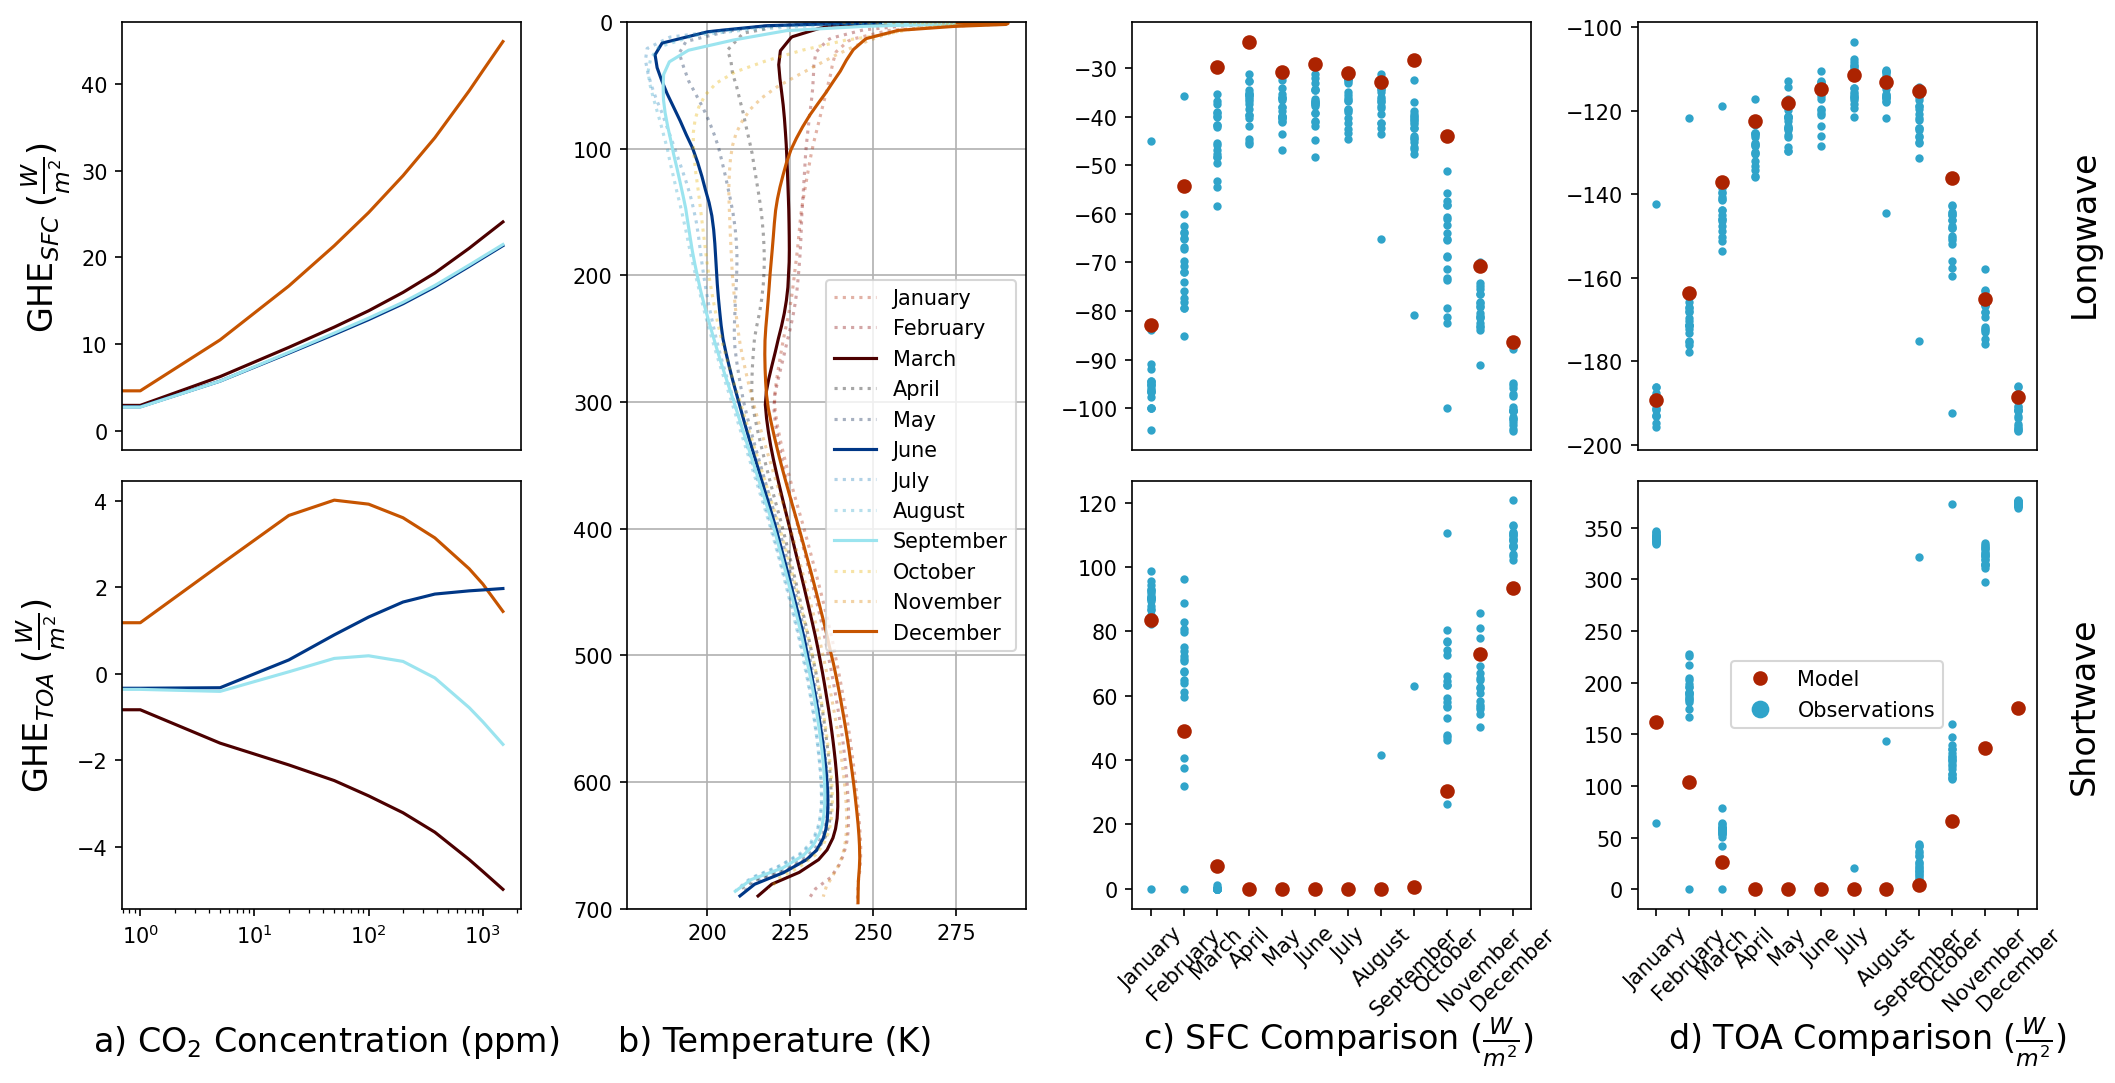
\includegraphics[width=1\textwidth]{figures/GH_sfc_CO2_effect.png}
\centering
\caption{}
\label{fig:sfc_toa_GHE}
\end{figure}

These are both shown in Figure \ref{fig:sfc_toa_GHE}, where we can see that the sign of ${\text{GHE}_{TOA}}$ is seasonally dependent, while the ${\text{GHE}_{SFC}}$ is always positive, independent of the time of year. This is in line with the conclusions of previous work, which finds positive radiative forcing by \ce{CO_2} and thus decreasing OLR during the winter (\cite{schmithusen_how_2015}). This increase in OLR with increasing \ce{CO_2} concentrations leads to increasing top-of-atmosphere (TOA) radiative loss under higher GHG scenarios during September-April. In order to better understand the relationship between our ${\text{GHE}_{SFC}}$ and surface temperatures, we rewrite our ${\text{GHE}_{SFC}}$ of \ce{CO_2} in terms of the Planck function and the bandwidth of \ce{CO_2}
\begin{equation}\label{eq:GHE_sfc}
    {\text{GHE}_{SFC}} = W(c)[\pi B(\nu,T_s)]
\end{equation}
where W(c) is the bandwidth, which we can then estimate based on (\cite{jeevanjee_analytical_2020}) as
\begin{equation}\label{eq:bandwidth}
    W(c) \approx 2\ell ln(\frac{C}{C_0})
\end{equation}
where $\pi B(\nu,T_s)$ is the Planck function based on a centered absorption band ($\nu$) of \ce{CO_2} at 667 cm$^-1$, $C_0$ is set to .25, C is the concentration of \ce{CO_2}, $\ell$, the spectroscopic decay parameter, is 10.4 cm$^{-1}$. We can compare both the bandwidth calculations and the subsequent ${\text{GHE}_{SFC}}$ calculations to our RRTMG model results, as seen in Figure \ref{fig:sfc_bandwidth_co2}. The estimated bandwidth does a good job of capturing the bandwidth throughout the year, with slight overestimates at lower \ce{CO_2} concentrations. This overestimate carries into the ${\text{GHE}_{SFC}}$ at lower \ce{CO_2} concentrations, but we can see that this estimate does a good job of capturing the general trend of the ${\text{GHE}_{SFC}}$ over different \ce{CO_2} concentrations. 


\begin{figure}[htb!]
\noindent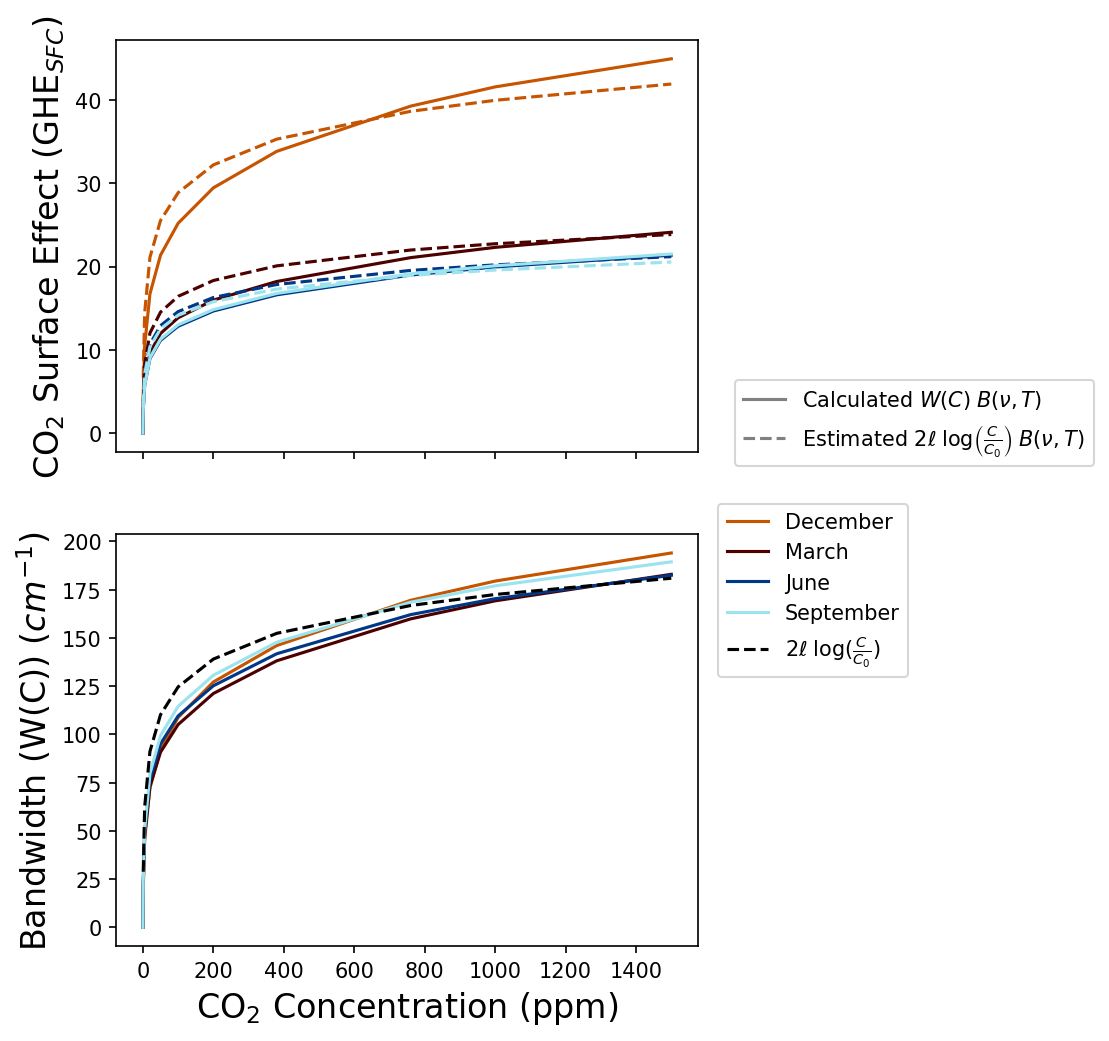
\includegraphics[width=1\textwidth]{figures/sfc_bandwidth_and_co2.png}
\centering
\caption{\ce{CO_2} surface effect (upper) and bandwidth (lower) across varying \ce{CO_2} concentrations from 0-1500 ppm for December, March, June and September. The \ce{CO_2} surface effect is calculated according to equation \ref{eq:GHE_sfc} (solid lines) as well as replacing the bandwidth in \ref{eq:GHE_sfc} with \ref{eq:bandwidth} (dashed lines). The bandwidth is similarly calculated based on \ref{eq:GHE_sfc} (solid lines), and estimated by \ref{eq:bandwidth} (dashed line).}
\label{fig:sfc_bandwidth_co2}
\end{figure}


\section{Radiative-Advective-Turbulent Model}
% Radiative-advective-turbulent calculations - methods + results (surface exchange + advection + time stepping all need to be documented)
% 3) \Delta T (2xCO2 - 1xCO2) for all months with sub-panels for surface T change

We build on this understanding of the relationship between the ${\text{GHE}_{SFC}}$ and what this means for surface temperature response to changes in \ce{CO_2} through expanding our model and time-stepping it to an equilibrium state. The model is composed of three parts: a radiative component, an advective component, and a turbulent component. The model computes temperature tendencies from the flux divergence of each component and steps the temperature forward in time according to:
\begin{equation}
    \rho c_{p} \pdv{T}{t} = -\nabla \cdot \mathbf{\mathcal{F}}
\end{equation}
The radiation component is calculated as described above using RRTMG, and the turbulent and advective components are added in order to represent turbulence in the planetary boundary layer and meridional advection. 

\subsubsection{Turbulence}
We construct a near-surface turbulence component based on the turbulent flux of potential temperature
\begin{equation}
    F_{turb} = -k(z) \frac{d\theta}{dz},
\end{equation}
where $k(z) = \overline{k_0} \exp(-\frac{z}{d})$ is an exponentially decaying diffusivity with a surface value of $k_0$ and a turbulence scale factor of $d = 100$ meters, which confines substantial turbulent fluxes to the bottom few model levels. We calculate $k_0$ diagnostically from the initial condition
\begin{equation}
    k_0^{(m)} = \frac{F_{\text{sfc, rad}}}{\frac{d\theta}{dz}_{\text{sfc}}},
\end{equation}
for each month $m$, where our radiative surface flux is calculated as
\begin{equation}
    F_{\text{sfc, rad}} = F_{\text{sfc, SW}} - F_{\text{sfc, LW}}.
\end{equation}

From this, we average the (nine) positive $k_0^{(m)}$ values, and use this as our final $\overline{k_0}$ throughout the experiments.

The turbulent heating rate is thus the flux divergence divided by the heat capacity of air and ice, for the atmosphere and surface, respectively:
\begin{equation}
    \text{HR}_{\text{turb}} = -\frac{\text{dF}_{\text{turb}}}{dz} /(c_p \rho).
\end{equation}

Our turbulence profiles vary across months, warming the surface during the winter and cooling it in the summer in order to balance the surface radiative heating rates.

\subsubsection{Advection}
We calculate our advective heating rate based on the initial state for each month at \ce{CO_2} = 380ppm, where it is set to balance the sum of the radiative and turbulent heating rates.

\begin{equation}
    \frac{dF_{adv}}{dz} = -(\frac{dF_{rad}}{dz} + \frac{dF_{turb}}{dz})\quad \text{at t = 0 and \ce{CO_2} = 380 ppm}
\end{equation}
The resulting advective heating rate is held constant throughout time, in order to allow us to isolate the adjustments of the radiative and turbulent components in time. 

We run the model forward for five months to assess the equilibrium state in our base and doubled \ce{CO_2} scenarios. At the equilibrium state, we evaluate the difference between a base (380 ppm) and a doubled (760 ppm) \ce{CO_2} scenario, finding that the doubled case has surface temperatures that range between 1.00 and 1.43 degrees warmer than that of the base scenario. On the other hand, the stratosphere in the double scenario cools relative to the base. Both this stratospheric cooling and surface temperature warming due to increases in \ce{CO_2} are similar to what is seen globally in regions without temperature inversions. This surface warming supports previous conclusions by (\cite{flanner_climate_2018}). This warming at the surface across all months and seasons can be best understood in relation to the $\text{GHE}_{SFC}$ rather than the $\text{GHE}_{TOA}$.

\begin{figure}[htb!]
\noindent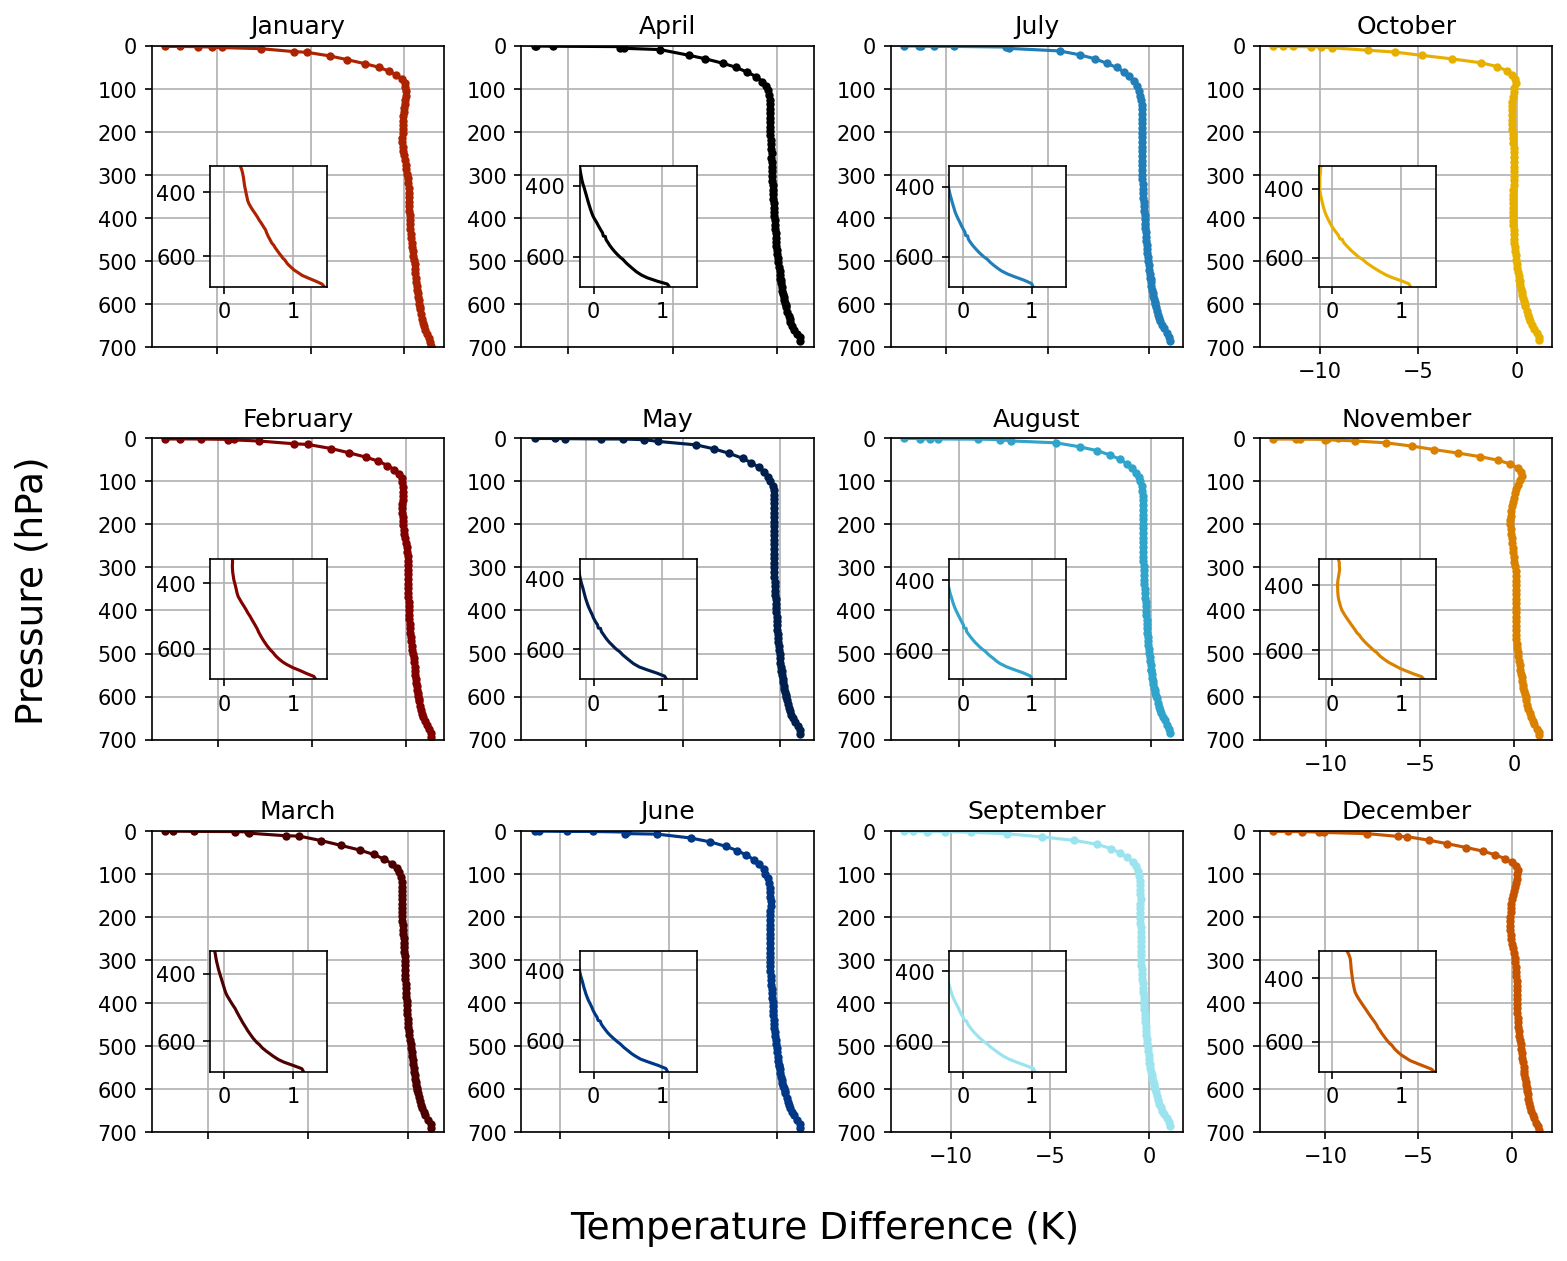
\includegraphics[width=1\textwidth]{figures/temp_dif.png}
\centering
\caption{Vertical profiles of equilibrium temperature differences between the double and base \ce{CO_2} scenario for each month resulting from our model. Insets show the bottom three hundred meters of temperature change to highlight the surface warming across all months.}
\label{fig:temp_dif}
\end{figure}


\section{Discussion and Conclusion} 
%
% Discussion 
% 4) predicted surface temperature change (relative to no CO2) compared to radiative-advective-turbulent model calculations (scatter plot)

Is there a simple way to understand the surface temperature change resulting from varying \ce{CO_2} in our simulations? Considering the perturbation surface radiative energy balance only, the increase in GHE$_{SFC}$, with increasing \ce{CO_2} concentration would need to be balanced by the additional upward longwave radiation from this warmer surface: $ 4 \sigma T_s^3 \delta T_s = \delta F_{\text{SFC}, \text{upward}}$, as can be derived from the Stefan-Boltzman law. This balance of upward longwave radiation from the warmer surface with the GHE$_{SFC}$ allows us to estimate the change in surface temperature due to a change in \ce{CO_2} forcing as: $\text{GHE}_{\text{SFC}} = 4 \sigma T_s^3 \delta T_s$. Where we can simplify this understanding as a function of the estimated bandwidth and planck function, utilizing our definition of GHE$_{SFC}$ from equation \ref{eq:GHE_sfc}.

\begin{equation}\label{eq:del_ts_planck}
    \delta T_s = \frac{2\ell log\frac{C}{C_0} [\pi B(\nu, T_s)]}{4\sigma T_s^3}
\end{equation}

We can see in Figure \ref{fig:delta_ts} that our equilibrium state change in surface temperature as predicted by the model can also be well understood by both of these estimations across multiple \ce{CO_2} concentrations. Particularly, the estimation from \ref{eq:del_ts_planck} allows us to calculate the change in temperature response to a varying degree of initial \ce{CO_2} concentrations with only an initial temperature state, an estimate of $C_0$, and an estimate of the central absorption band for \ce{CO_2} ($\nu$). In the case where values for 

Using a radiative-advective-turbulent single column model, we are able to establish a relationship between the surface temperature changes in the Antarctic and the upward surface flux across multiple \ce{CO_2} concentrations. The \ce{CO_2} surface effect is positive across all months, and increases with \ce{CO_2} concentrations. In contrast to the OLR impacts of changing \ce{CO_2} concentrations, this framework allows for a simplified calculation of the change in surface temperature based only on an initial surface temperature, and change in \ce{CO_2} concentration. 

\begin{figure}[htb!]
\noindent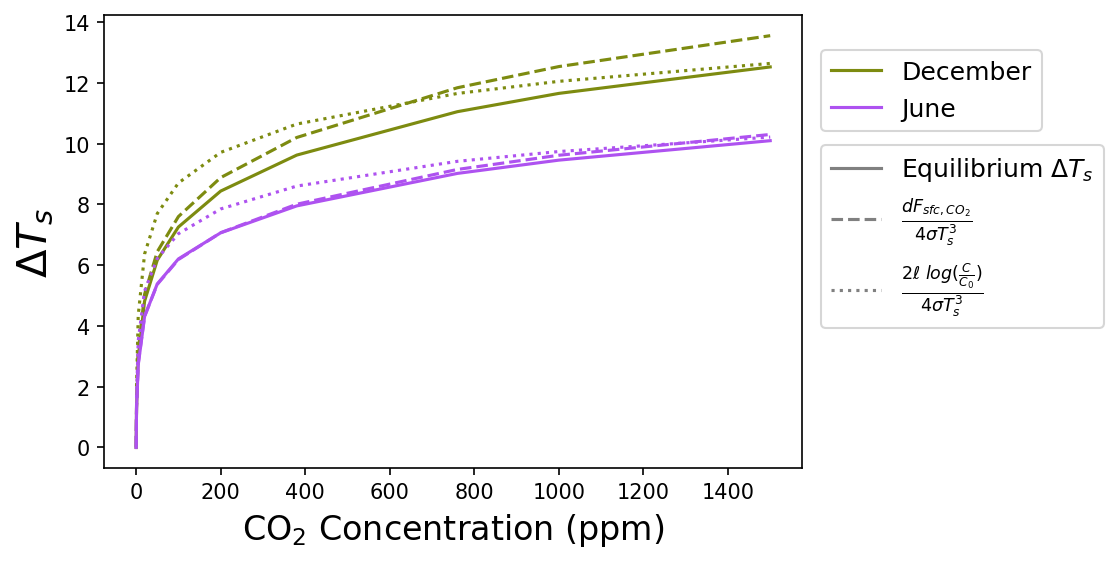
\includegraphics[width=1\textwidth]{figures/delta_Ts.png}
\centering
\caption{Surface temperature change from the initial to equilibrium state for the months of June and December across different \ce{CO_2} values, ranging from 0-1500 ppm. The solid lines depict the difference in equilibrium surface temperature from our single column model; dashed lines indicate the estimated temperature difference based on the derivative of the Stefan-Boltzman law; dotted lines indicated the estimated temperature difference based on equation \ref{eq:del_ts_planck}. Estimations from equation \ref{eq:del_ts_planck} overestimate at low \ce{CO_2} concentrations, while accuracy of estimations from the Stefan Boltzman law vary based on the season.}
\label{fig:delta_ts}
\end{figure}

%%

%  Numbered lines in equations:
%  To add line numbers to lines in equations,
%  \begin{linenomath*}
%  \begin{equation}
%  \end{equation}
%  \end{linenomath*}



%% Enter Figures and Tables near as possible to where they are first mentioned:
%
% DO NOT USE \psfrag or \subfigure commands.
%
% Figure captions go below the figure.
% Table titles go above tables;  other caption information
%  should be placed in last line of the table, using
% \multicolumn2l{$^a$ This is a table note.}
%
%----------------
% EXAMPLE FIGURES
%
% \begin{figure}
% \includegraphics{example.png}
% \caption{caption}
% \end{figure}
%
% Giving latex a width will help it to scale the figure properly. A simple trick is to use \textwidth. Try this if large figures run off the side of the page.
% \begin{figure}
% \noindent\includegraphics[width=\textwidth]{anothersample.png}
%\caption{caption}
%\label{pngfiguresample}
%\end{figure}
%
%
% If you get an error about an unknown bounding box, try specifying the width and height of the figure with the natwidth and natheight options. This is common when trying to add a PDF figure without pdflatex.
% \begin{figure}
% \noindent\includegraphics[natwidth=800px,natheight=600px]{samplefigure.pdf}
%\caption{caption}
%\label{pdffiguresample}
%\end{figure}
%
%
% PDFLatex does not seem to be able to process EPS figures. You may want to try the epstopdf package.
%

%
% ---------------
% EXAMPLE TABLE
%
% \begin{table}
% \caption{Time of the Transition Between Phase 1 and Phase 2$^{a}$}
% \centering
% \begin{tabular}{l c}
% \hline
%  Run  & Time (min)  \\
% \hline
%   $l1$  & 260   \\
%   $l2$  & 300   \\
%   $l3$  & 340   \\
%   $h1$  & 270   \\
%   $h2$  & 250   \\
%   $h3$  & 380   \\
%   $r1$  & 370   \\
%   $r2$  & 390   \\
% \hline
% \multicolumn{2}{l}{$^{a}$Footnote text here.}
% \end{tabular}
% \end{table}

%% SIDEWAYS FIGURE and TABLE
% AGU prefers the use of {sidewaystable} over {landscapetable} as it causes fewer problems.
%
% \begin{sidewaysfigure}
% \includegraphics[width=20pc]{figsamp}
% \caption{caption here}
% \label{newfig}
% \end{sidewaysfigure}
%
%  \begin{sidewaystable}
%  \caption{Caption here}
% \label{tab:signif_gap_clos}
%  \begin{tabular}{ccc}
% one&two&three\\
% four&five&six
%  \end{tabular}
%  \end{sidewaystable}

%% If using numbered lines, please surround equations with \begin{linenomath*}...\end{linenomath*}
%\begin{linenomath*}
%\begin{equation}
%y|{f} \sim g(m, \sigma),
%\end{equation}
%\end{linenomath*}

%%% End of body of article

%%%%%%%%%%%%%%%%%%%%%%%%%%%%%%%%
%% Optional Appendix goes here
%
% The \appendix command resets counters and redefines section heads
%
% After typing \appendix
%
%\section{Here Is Appendix Title}
% will show
% A: Here Is Appendix Title
%
%\appendix
%\section{Here is a sample appendix}

%%%%%%%%%%%%%%%%%%%%%%%%%%%%%%%%%%%%%%%%%%%%%%%%%%%%%%%%%%%%%%%%
%
% Optional Glossary, Notation or Acronym section goes here:
%
%%%%%%%%%%%%%%
% Glossary is only allowed in Reviews of Geophysics
%  \begin{glossary}
%  \term{Term}
%   Term Definition here
%  \term{Term}
%   Term Definition here
%  \term{Term}
%   Term Definition here
%  \end{glossary}

%
%%%%%%%%%%%%%%
% Acronyms
%   \begin{acronyms}
%   \acro{Acronym}
%   Definition here
%   \acro{EMOS}
%   Ensemble model output statistics
%   \acro{ECMWF}
%   Centre for Medium-Range Weather Forecasts
%   \end{acronyms}

%
%%%%%%%%%%%%%%
% Notation
%   \begin{notation}
%   \notation{$a+b$} Notation Definition here
%   \notation{$e=mc^2$}
%   Equation in German-born physicist Albert Einstein's theory of special
%  relativity that showed that the increased relativistic mass ($m$) of a
%  body comes from the energy of motion of the body—that is, its kinetic
%  energy ($E$)—divided by the speed of light squared ($c^2$).
%   \end{notation}




%%%%%%%%%%%%%%%%%%%%%%%%%%%%%%%%%%%%%%%%%%%%%%%%%%%%%%%%%%%%%%%%
%
%  ACKNOWLEDGMENTS
%
% The acknowledgments must list:
%
% >>>>	A statement that indicates to the reader where the data
% 	supporting the conclusions can be obtained (for example, in the
% 	references, tables, supporting information, and other databases).
%
% 	All funding sources related to this work from all authors
%
% 	Any real or perceived financial conflicts of interests for any
%	author
%
% 	Other affiliations for any author that may be perceived as
% 	having a conflict of interest with respect to the results of this
% 	paper.
%
%
% It is also the appropriate place to thank colleagues and other contributors.
% AGU does not normally allow dedications.


\acknowledgments
Enter acknowledgments, including your data availability statement, here.


%% ------------------------------------------------------------------------ %%
%% References and Citations

%%%%%%%%%%%%%%%%%%%%%%%%%%%%%%%%%%%%%%%%%%%%%%%
%
% \bibliography{<name of your .bib file>} don't specify the file extension
%
% don't specify bibliographystyle
%%%%%%%%%%%%%%%%%%%%%%%%%%%%%%%%%%%%%%%%%%%%%%%

\bibliography{references.bib}



%Reference citation instructions and examples:
%
% Please use ONLY \cite and \citeA for reference citations.
% \cite for parenthetical references
% ...as shown in recent studies (Simpson et al., 2019)
% \citeA for in-text citations
% ...Simpson et al. (2019) have shown...
%
%
%...as shown by \citeA{jskilby}.
%...as shown by \citeA{lewin76}, \citeA{carson86}, \citeA{bartoldy02}, and \citeA{rinaldi03}.
%...has been shown \cite{jskilbye}.
%...has been shown \cite{lewin76,carson86,bartoldy02,rinaldi03}.
%... \cite <i.e.>[]{lewin76,carson86,bartoldy02,rinaldi03}.
%...has been shown by \cite <e.g.,>[and others]{lewin76}.
%
% apacite uses < > for prenotes and [ ] for postnotes
% DO NOT use other cite commands (e.g., \citet, p, \citeyear, \nocite, \citealp, etc.).
%



\end{document}



More Information and Advice:

%% ------------------------------------------------------------------------ %%
%
%  SECTION HEADS
%
%% ------------------------------------------------------------------------ %%

% Capitalize the first letter of each word (except for
% prepositions, conjunctions, and articles that are
% three or fewer letters).

% AGU follows standard outline style; therefore, there cannot be a section 1 without
% a section 2, or a section 2.3.1 without a section 2.3.2.
% Please make sure your section numbers are balanced.
% ---------------
% Level 1 head
%
% Use the \section{} command to identify level 1 heads;
% type the appropriate head wording between the curly
% brackets, as shown below.
%
%An example:
%\section{Level 1 Head: Introduction}
%
% ---------------
% Level 2 head
%
% Use the \subsection{} command to identify level 2 heads.
%An example:
%\subsection{Level 2 Head}
%
% ---------------
% Level 3 head
%
% Use the \subsubsection{} command to identify level 3 heads
%An example:
%\subsubsection{Level 3 Head}
%
%---------------
% Level 4 head
%
% Use the \subsubsubsection{} command to identify level 3 heads
% An example:
%\subsubsubsection{Level 4 Head} An example.
%
%% ------------------------------------------------------------------------ %%
%
%  IN-TEXT LISTS
%
%% ------------------------------------------------------------------------ %%
%
% Do not use bulleted lists; enumerated lists are okay.
% \begin{enumerate}
% \item
% \item
% \item
% \end{enumerate}
%
%% ------------------------------------------------------------------------ %%
%
%  EQUATIONS
%
%% ------------------------------------------------------------------------ %%

% Single-line equations are centered.
% Equation arrays will appear left-aligned.

%Math coded inside display math mode \[ ...\]
% will not be numbered, e.g.,:
% \[ x^2=y^2 + z^2\]

 %Math coded inside \begin{equation} and \end{equation} will
% be automatically numbered, e.g.,:
 %\begin{equation}
 %x^2=y^2 + z^2
 %\end{equation}


% To create multiline equations, use the
% \begin{eqnarray} and \end{eqnarray} environment
% as demonstrated below.
%\begin{eqnarray}
 % x_{1} & = & (x - x_{0}) \cos \Theta \nonumber \\
  %      && + (y - y_{0}) \sin \Theta  \nonumber \\
  %y_{1} & = & -(x - x_{0}) \sin \Theta \nonumber \\
  %      && + (y - y_{0}) \cos \Theta.
%\end{eqnarray}

%If you don't want an equation number, use the star form:
%\begin{eqnarray*}...\end{eqnarray*}

% Break each line at a sign of operation
% (+, -, etc.) if possible, with the sign of operation
% on the new line.

% Indent second and subsequent lines to align with
% the first character following the equal sign on the
% first line.

% Use an \hspace{} command to insert horizontal space
% into your equation if necessary. Place an appropriate
% unit of measure between the curly braces, e.g.
% \hspace{1in}; you may have to experiment to achieve
% the correct amount of space.


%% ------------------------------------------------------------------------ %%
%
%  EQUATION NUMBERING: COUNTER
%
%% ------------------------------------------------------------------------ %%

% You may change equation numbering by resetting
% the equation counter or by explicitly numbering
% an equation.

% To explicitly number an equation, type \eqnum{}
% (with the desired number between the brackets)
% after the \begin{equation} or \begin{eqnarray}
% command.  The \eqnum{} command will affect only
% the equation it appears with; LaTeX will number
% any equations appearing later in the manuscript
% according to the equation counter.
%

% If you have a multiline equation that needs only
% one equation number, use a \nonumber command in
% front of the double backslashes (\\) as shown in
% the multiline equation above.

% If you are using line numbers, remember to surround
% equations with \begin{linenomath*}...\end{linenomath*}

%  To add line numbers to lines in equations:
%  \begin{linenomath*}
%  \begin{equation}
%  \end{equation}
%  \end{linenomath*}



